\documentclass{article}

\usepackage{amsmath}
\usepackage{graphicx}

\author{Elliot O. Cornier}
\date{\today}

\begin{document}
\section{Pre-lab design}
\subsection{Question D1}
The following model describes the changes in electrical resistance as a function of strain:
\begin{equation}
    \epsilon = \frac{dR}{RG'}
\end{equation}
Where:
\begin{itemize}
    \item \(\epsilon\) represents strain factor
    \item \(R\) is the nominal resistance
    \item \(dR\) is the change in resistance
    \item \(G\) is the gauge factor.
\end{itemize}
Calculate the change in resistance \(dR\) if \(R=120\Omega\), \(G=2\) and \(\epsilon=0.01\):
\begin{equation}
    \begin{aligned}
        dR&=\epsilon RG' \\
        dR&=0.01 \cdot 120\Omega \cdot 2 \\
        dR&=2.4\Omega
    \end{aligned}
\end{equation}

\subsection{Question D2}
\begin{figure}[ht]
    \centering
    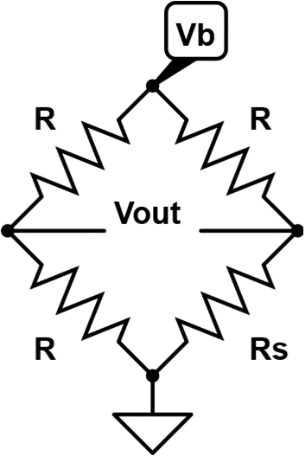
\includegraphics[width=0.3\textwidth]{images/wheatstone bridge.png}
    \caption{Wheatstone bridge.}
    \label{fig:wheatstone}
\end{figure}
Let the strain gauge resistance be represented by \(Rs\):
\begin{equation}
    Rs=R+dR
\end{equation}
Let the other three resistors have the same nominal resistance \(Rs\) as the strain gauge. 
The expression for \(V_{out}\) becomes:
\begin{equation}
    \begin{aligned}
        V_{out}&=V_b \cdot \frac{R}{R+R} - V_b \cdot \frac{Rs}{Rs+R} \\
        V_{out}&=V_b \left( \frac{1}{2} - \frac{Rs}{Rs + R} \right) \\
        V_{out}&=V_b \left( \frac{1}{2} - \frac{R+dR}{2R+dR} \right)
    \end{aligned}
\end{equation}

\subsection{Question D3}
Consider \(V_b=5V\), \(R=120\Omega\), calculate \(V_{out}\) for a 1\% strain:
\begin{equation}
    \begin{aligned}
        V_{out}&=V_b \cdot \frac{R}{R+R} - V_b \cdot \frac{Rs}{Rs+R} \\
        V_{out}&=5V \cdot \frac{120\Omega}{240\Omega} - 5V \cdot \frac{120\Omega + 2.4\Omega}{120\Omega + 120\Omega + 2.4\Omega} \\
        V_{out}&= 5V \left( \frac{1}{2} - \frac{122.4\Omega}{242.4\Omega} \right) \\
        V_{out}&= -0.02475V
    \end{aligned}
\end{equation}
Re-calculate now where each bridge resistor features \(R=114\Omega\):
\begin{equation}
    \begin{aligned}
        V_{out}&=V_b \cdot \frac{R}{R+R} - V_b \cdot \frac{Rs}{Rs+R} \\
        V_{out}&=5V \cdot \frac{114\Omega}{114\Omega} - 5V \cdot \frac{120\Omega + 2.4\Omega}{120\Omega + 114\Omega + 2.4\Omega} \\
        V_{out}&= 5V \left( \frac{1}{2} - \frac{122.4\Omega}{236.4\Omega} \right) \\
        V_{out}&= -0.08883V
    \end{aligned}
\end{equation}

\newpage

\subsection{Question D4}
\begin{figure}[ht]
    \centering
    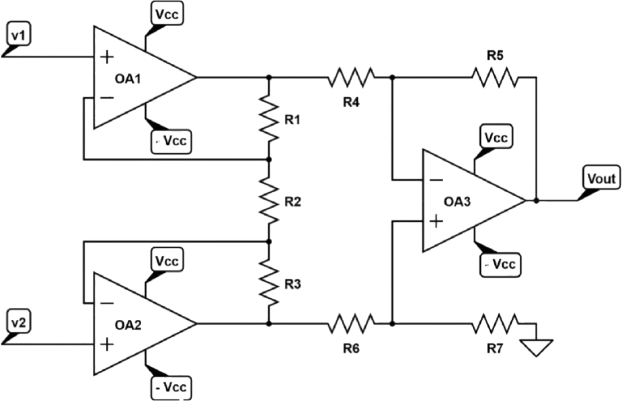
\includegraphics[width=1.0\textwidth]{images/instrumentation_amplifier.png}
    \caption{Instrumentation amplifier.}
    \label{fig:intsrumentation_amplifier}
\end{figure}

We wish to find an expression for \(\frac{V_{out}}{V_{in}}\), Let us denote \(V_{OA1},\quad V_{OA2}\) as opamp 1 and 2's output voltages respectively:
\begin{equation}
    I_{R2} = \frac{V_1 - V_2}{R2}
\end{equation}
Notice that the current must be equal for \(I_{R1} = I_{R2} = I_{R3}\), therefore:
\begin{equation}
    \begin{aligned}
        I_{R1} &= \frac{V_{OA1} - V_1}{R1} \\
        V_{OA1} - V_1 &= I_{R1} \cdot R1 \\
        V_{OA1} &= I_{R1} \cdot R1 + V_1 \\
        V_{OA1} &= \frac{V_1 - V_2}{R2} \cdot R1 + V_1
    \end{aligned}
\end{equation}
This can similarly be repeated for \(V_{OA2}\) to get:
\begin{equation}
    \begin{aligned}
        I_{R3} &= \frac{V_2 - V_{OA2}}{R3} \\
        V_2 - V_{OA2} &= I_{R3} \cdot R3 \\
        V_{OA2} &= V_2 - I_{R3} \cdot R3 \\
        V_{OA2} &= V_2 - \frac{V_1 - V_2}{R2} \cdot R3
    \end{aligned}
\end{equation}
Let us denote the inputs of the final op-amp as \(V_{+}, \quad V_{-}\), we then get:
\begin{equation}
    \begin{aligned}
        V_- = V_+ \\
        V_+ = V_{OA2} \cdot \frac{R7}{R6+R7} \\
        \text{KCL \@ Node V-} \\
        \frac{V_{OA1}-V_-}{R4} - \frac{V_- - V_{out}}{R5} = 0 \\
        \frac{V_{OA1}- V_-}{R4}=\frac{V_- - V_{out}}{R5} \\
        V_- - V_{out} = R5 \cdot \frac{V_{OA1 - V_-}}{R4} \\
        V_{out} = V_- - R5 \cdot \frac{V_{OA1} - V_-}{R4} \\ 
        V_{out} = \left( V_2 - \frac{V_1 - V_2}{R2} \cdot R3 \right) \cdot \frac{R7}{R6+R7} - R5 \cdot \frac{\left( \frac{V_1 - V_2}{R2} \cdot R1 + V_1 \right) - \left( \left( V_2 - \frac{V_1 - V_2}{R2} \cdot R3 \right) \cdot \frac{R7}{R6+R7} \right)}{R4}
    \end{aligned}
\end{equation}
\end{document}